%% DESIGN: Raleway | Bold/disruptive, unconventional layout | Orange (#E65100) accent
\documentclass[11pt,a4paper]{article}
\usepackage[left=0.5in,right=0.5in,top=0.4in,bottom=0.4in]{geometry}
\usepackage[T1]{fontenc}
\usepackage[thin]{raleway}
\usepackage{xcolor,titlesec,enumitem,hyperref,tikz,multicol}

\definecolor{accent}{HTML}{E65100}
\definecolor{ACCENT}{HTML}{E65100}
\definecolor{dark}{HTML}{1A1A1A}
\hypersetup{colorlinks=true,urlcolor=accent}
\pagestyle{empty}

\titleformat{\section}{\large\bfseries\color{accent}}{}{0em}{\MakeUppercase}[]
\titlespacing{\section}{0pt}{0.8em}{0.3em}

\begin{document}

% Bold unconventional header - diagonal stripe
\noindent
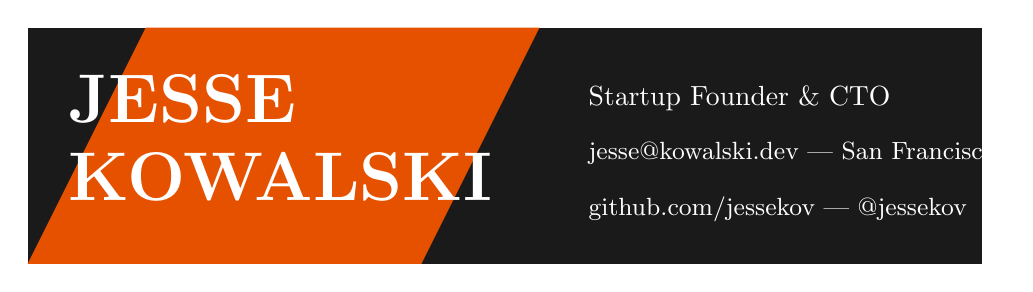
\begin{tikzpicture}
\fill[dark] (0,0) rectangle (\textwidth,3);
\fill[accent] (0,0) -- (5,0) -- (6.5,3) -- (1.5,3) -- cycle;
\node[anchor=west,text=white,font=\Huge\bfseries] at (0.4,2.1) {JESSE};
\node[anchor=west,text=white,font=\Huge\bfseries] at (0.4,1.1) {KOWALSKI};
\node[anchor=west,text=white!80,font=\normalsize] at (7,2.1) {Startup Founder \& CTO};
\node[anchor=west,text=white!60,font=\small] at (7,1.4) {jesse@kowalski.dev | San Francisco};
\node[anchor=west,text=white!60,font=\small] at (7,0.7) {github.com/jessekov | @jessekov};
\end{tikzpicture}

\vspace{0.5em}

\begin{multicols}{2}

\section{The Short Version}
Serial technical founder. Built 2 startups from zero to acquisition. Write code, hire teams, raise capital, close deals. Currently building the future of developer tools.

\section{Founded}

\noindent{\large\bfseries\color{accent} DevForge} {\small (2022--Present)}\\
\textit{AI-powered developer productivity platform}
\begin{itemize}[leftmargin=0.8em,nosep,label={\color{accent}\textbf{/}}]
\item Raised \$12M Series A (a16z, First Round)
\item 50K+ developers, \$3M ARR in 18 months
\item Built team of 25 engineers
\item Architected core platform (Rust + TypeScript)
\end{itemize}
\vspace{0.4em}

\noindent{\large\bfseries\color{accent} CodeShip} {\small (2018--2022, acquired)}\\
\textit{CI/CD platform for ML teams}
\begin{itemize}[leftmargin=0.8em,nosep,label={\color{accent}\textbf{/}}]
\item Acquired by DataDog for \$28M (2022)
\item Grew to 200+ enterprise customers
\item Team of 15; \$5M ARR at exit
\item Led all technical architecture decisions
\end{itemize}

\columnbreak

\section{Before Founding}

\noindent\textbf{Staff Engineer} \hfill \textcolor{accent}{2015--2018}\\
\textit{Stripe, San Francisco}
\begin{itemize}[leftmargin=0.8em,nosep,label={\color{accent}\textbf{/}}]
\item Led payments infrastructure team (8 eng)
\item Designed system processing \$10B+ annually
\item 3 patents in distributed systems
\end{itemize}
\vspace{0.4em}

\noindent\textbf{Senior SDE} \hfill \textcolor{accent}{2013--2015}\\
\textit{Google, Mountain View}
\begin{itemize}[leftmargin=0.8em,nosep,label={\color{accent}\textbf{/}}]
\item Core contributor to Kubernetes (early team)
\item Built internal deployment tooling
\end{itemize}

\section{Tech I Ship With}
\noindent Rust, Go, TypeScript, Python\\
Kubernetes, AWS, Terraform\\
PostgreSQL, Redis, Kafka\\
React, Next.js, Tailwind

\section{Education}
\noindent\textbf{B.S. CS} \hfill Stanford, 2013\\
{\small (Dropped out of MS to join Google)}

\section{Talks \& Writing}
\begin{itemize}[leftmargin=0.8em,nosep,label={\color{accent}\textbf{/}}]
\item ``Scaling from 0 to 1'' -- YC Startup School
\item ``Technical Founders Guide'' -- 50K readers
\item KubeCon keynote 2023
\end{itemize}

\end{multicols}

\end{document}
